\documentclass{article}
\usepackage{amsmath}
\usepackage{amssymb}
\usepackage{algorithmic}
\usepackage{algorithm}
\usepackage{hyperref}
\usepackage{tikz}
\usetikzlibrary{arrows.meta,positioning,shapes.geometric}

\title{Futarchy AMMs: Quantum Liquidity, Pass-Through Oracles, and Atomic Market Initialization}
\author{Greshams Code\\Govex.ai}
\date{September 2025}

\begin{document}

\maketitle

\begin{abstract}
We present three novel mechanisms for futarchy prediction markets: (1) \textbf{Quantum liquidity flow}, where spot tokens split into full-value conditional tokens across all outcomes simultaneously, enabling Hanson-style futarchy with efficient capital usage; (2) \textbf{Pass-through oracles}, maintaining price continuity across state transitions via transparent proxying and retroactive gap-filling; (3) \textbf{Atomic market initialization}, allowing instant proposal creation with encrypted asymmetric liquidity seeding for front-run-proof price signaling. Together, these achieve continuous price discovery with $O(1)$ storage overhead while enabling DAOs to express market beliefs atomically.
\end{abstract}

\section{Introduction}

Futarchy—governance by prediction markets—requires efficient mechanisms for:
\begin{itemize}
\item Capital efficiency: Liquidity must exist simultaneously across outcome markets
\item Price continuity: Oracles must maintain smooth readings across state transitions
\item Strategic signaling: DAOs must seed markets without revealing parameters to front-runners
\end{itemize}

Traditional AMMs fail these requirements. We present a unified architecture solving all three.

\section{Part I: Quantum Liquidity Flow}

\subsection{Hanson-Style Futarchy Model}

Let $L_{spot}$ be spot AMM liquidity. In traditional designs, conditional markets split this proportionally. We instead use \textbf{quantum splitting}:

$$L_{spot} \xrightarrow{\text{split}} \{L_1, L_2, ..., L_n\} \text{ where } L_i = L_{spot} \; \forall i$$

Each conditional market receives \emph{full} liquidity, not a fraction.

\textbf{Key insight:} Only the highest-priced outcome wins. Tokens in losing outcomes become worthless, so quantum superposition collapses to single outcome.

\subsection{Token Mechanics}

Define conditional token minting:
$$1 \text{ SPOT} \to 1 \text{ COND}_i \quad \forall i \in \{1,...,n\}$$

Redemption (winning outcome $w$ only):
$$1 \text{ COND}_w \to 1 \text{ SPOT}$$

For binary markets: $P_{yes} + P_{no} = 1$ (constant sum).

\subsection{Liquidity State Machine}

\begin{center}
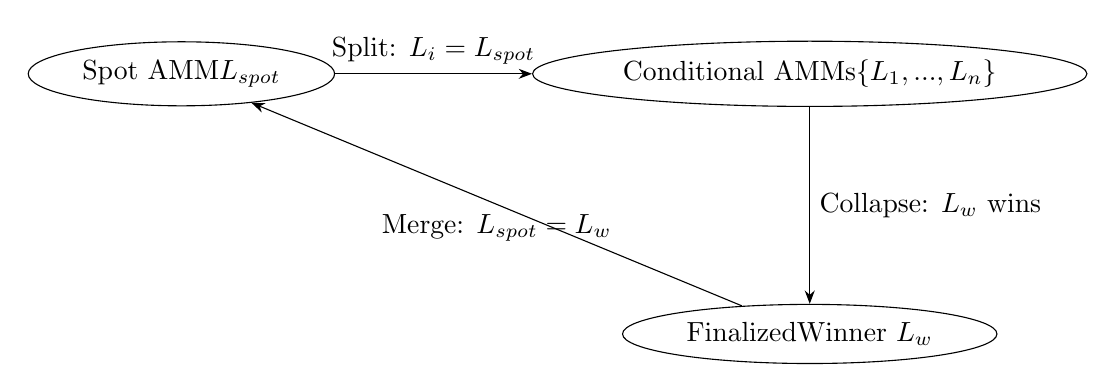
\begin{tikzpicture}[node distance=2.5cm, auto, >=Stealth]
  \node[ellipse, draw] (spot) {Spot AMM\\$L_{spot}$};
  \node[ellipse, draw, right=of spot] (cond) {Conditional AMMs\\$\{L_1, ..., L_n\}$};
  \node[ellipse, draw, below=of cond] (final) {Finalized\\Winner $L_w$};

  \draw[->] (spot) -- node[above] {Split: $L_i = L_{spot}$} (cond);
  \draw[->] (cond) -- node[right] {Collapse: $L_w$ wins} (final);
  \draw[->] (final) -- node[below] {Merge: $L_{spot} = L_w$} (spot);
\end{tikzpicture}
\end{center}

\textbf{During proposals:} Spot AMM is \emph{completely empty}. All liquidity exists quantum-mechanically in conditional markets.

\subsection{Price Discovery Across Outcomes}

Spot price during proposal is undefined. Instead:
$$P_{effective}(\tau) = \max_{i \in \{1,...,n\}} P_i(\tau)$$

where $P_i(\tau)$ is conditional AMM $i$'s spot price.

\textbf{Security property:} Manipulating requires attacking \emph{all} conditional markets simultaneously.

\section{Part II: Pass-Through Oracles}

\subsection{Problem Formulation}

Let $\mathcal{S} = \{s_0, s_1, ..., s_n\}$ be system states where $s_0$ represents spot trading and $s_i$ for $i > 0$ represents conditional trading for outcome $i$.

\textbf{Time notation:}
\begin{itemize}
\item $t_{start}$: Proposal starts (liquidity splits to conditional)
\item $t_{end}$: Proposal ends (liquidity merges back)
\item $t_{init}$: Oracle initialization time
\item $t_{last}$: Last observation/update time
\item $\tau$: Query time (current time when TWAP requested)
\item $\Delta t$: Discrete time step between observations
\end{itemize}

\textbf{Price notation:}
\begin{itemize}
\item $P(k)$: Spot price at discrete time $k$
\item $P_{conditional}(k)$: Conditional price at time $k$
\item $P_{last}$: Last observed price
\item $C_{spot}(t)$: Cumulative spot price up to time $t$
\item $C_{combined}$: Combined cumulative during proposal
\item $W$: TWAP window duration
\item $W_{eff}$: Effective window (accounting for initialization)
\end{itemize}

Define oracle function:
$$O_t: \mathcal{S} \times [0, \infty) \to \mathbb{R}^+$$

where $O_t(s, \tau)$ returns TWAP at time $\tau$ for state $s$.

\textbf{Discontinuity Problem:} At state transition $t_{trans}$:
$$\lim_{\tau \to t_{trans}^-} O_t(s_0, \tau) \neq \lim_{\tau \to t_{trans}^+} O_t(s_i, \tau)$$

\subsection{Pass-Through Mechanism}

Define pass-through oracle $\hat{O}_t$ as:

$$\hat{O}_t(\tau) = \begin{cases}
O_t(s_0, \tau) & \text{if } \tau < t_{start} \\
O_t(s_{w(\tau)}, \tau) & \text{if } t_{start} \leq \tau < t_{end} \\
O_t(s_0, \tau) & \text{if } \tau \geq t_{end}
\end{cases}$$

where $w(\tau) = \arg\max_{i} P_i(\tau)$ (winning outcome = highest price).

\subsection{Retroactive Gap Filling}

Upon finalization at $t_{end}$, update spot oracle's cumulative price:

$$C_{s_0}(t_{end}) = C_{s_0}(t_{start}) + \sum_{k=t_{start}}^{t_{end}-1} P_{s_w}(k) \cdot \Delta t$$

where $P_{s_w}(k)$ is price from winning conditional AMM at discrete time $k$.

\subsection{Window Management}

For rolling window of duration $W$, effective TWAP at time $\tau$:

$$\text{TWAP}(\tau) = \frac{1}{W_{eff}} \sum_{k=\max(\tau - W, t_{init})}^{\tau-1} P(k) \cdot \Delta t$$

where $W_{eff} = \min(W, \tau - t_{init})$.

During proposal ($t_{start} \leq \tau < t_{end}$):

$$\text{TWAP}(\tau) = \frac{C_{spot}(t_{start}) + \sum_{k=t_{start}}^{\tau-1} P_{w(k)}(k) \cdot \Delta t}{W_{eff}}$$

\subsection{Implementation}

\begin{algorithm}
\caption{Pass-Through Oracle Read}
\begin{algorithmic}
\STATE \textbf{function} GetTWAP($\tau$: query time)
\IF{proposal\_active}
    \STATE $w \gets \arg\max_i P_i(\tau)$ \COMMENT{Find winning outcome}
    \STATE $n_{steps} \gets \lfloor(\tau - t_{start}) / \Delta t\rfloor$
    \STATE $C_{combined} \gets C_{spot}(t_{start}) + P_w \cdot n_{steps} \cdot \Delta t$
    \STATE $W_{eff} \gets \min(W, \tau - t_{init})$
    \RETURN $C_{combined} / W_{eff}$
\ELSE
    \STATE $n_{steps} \gets \lfloor(\tau - t_{last}) / \Delta t\rfloor$
    \STATE $C_{projected} \gets C_{spot}(t_{last}) + P_{last} \cdot n_{steps} \cdot \Delta t$
    \STATE $W_{eff} \gets \min(W, \tau - t_{init})$
    \RETURN $C_{projected} / W_{eff}$
\ENDIF
\end{algorithmic}
\end{algorithm}

\subsection{Dual Oracle Architecture}

We employ two complementary oracles:

\subsubsection{Write-Through TWAP (Governance)}
From \cite{twap2025}, with retroactive step adjustments:
$$P'_i = B + \text{sign}(P-B) \cdot \min(i \cdot \Delta_M, |P-B|)$$

Requires mutation before read, preventing stale prices.

\subsubsection{Ring Buffer Oracle (External)}
Adapted from Uniswap V3 \cite{uniswapv3}:

\begin{algorithm}
\caption{Ring Buffer Write}
\begin{algorithmic}
\STATE $idx \gets (current + 1) \mod capacity$
\STATE $observations[idx] \gets \{timestamp, cumulative, price\}$
\STATE $current \gets idx$
\end{algorithmic}
\end{algorithm}

Key adaptation: \texttt{merge\_observations()} for seamless history integration:

$$O_{merged} = O_{spot} \cup \{o \in O_{conditional} : t_{start} \leq o.t \leq t_{end}\}$$

\subsection{Properties}

\subsubsection{Continuity}
\begin{theorem}
The pass-through oracle maintains $C^0$ continuity:
$$\forall t: \lim_{\tau \to t^-} \hat{O}_t(\tau) = \lim_{\tau \to t^+} \hat{O}_t(\tau)$$
\end{theorem}

\begin{proof}
At $t_{start}$: Both oracles initialized from same spot price $P_0$:
$$\lim_{\tau \to t_{start}^-} \hat{O}_t(\tau) = P_0 = \lim_{\tau \to t_{start}^+} \hat{O}_t(\tau)$$

At $t_{end}$: Gap-filling ensures:
$$C_{spot}(t_{end}^+) = C_{spot}(t_{start}) + \sum_{k=t_{start}}^{t_{end}-1} P_{conditional}(k) \cdot \Delta t$$

Thus: $\lim_{\tau \to t_{end}^-} \hat{O}_t(\tau) = \lim_{\tau \to t_{end}^+} \hat{O}_t(\tau)$

During proposal: Direct read from winning conditional ensures no jumps.
\end{proof}

\subsubsection{Manipulation Resistance}
Cost to manipulate by $\delta$:
$$C_{manip} = \sum_{i=1}^{n} \frac{L_i \cdot \delta^2}{2(1-\delta)}$$

Pass-through preserves this as manipulation must occur in active oracle (spot or winning conditional).

\section{Part III: Atomic Market Initialization}

\subsection{Problem: Front-Running Market Seeding}

DAOs want to seed markets with asymmetric liquidity to signal beliefs. Naive approach:
\begin{enumerate}
\item Create proposal
\item Wait for markets to form
\item Execute trades to seed liquidity
\end{enumerate}

\textbf{Attack:} Front-runners see pending trades and extract value.

\subsection{Solution: Atomic PTB Execution}

All operations in single transaction:
\begin{enumerate}
\item Create proposal (PREMARKET state)
\item Create escrow + conditional AMMs
\item Execute DAO intent (mint or withdraw)
\item Execute market init strategy
\item Return proceeds to DAO vault
\item Finalize proposal (→ REVIEW/TRADING)
\end{enumerate}

\textbf{No intermediate state exposed} → front-run proof.

\subsection{Market Initialization Strategies}

\subsubsection{Conditional Raise (Mint + Sell)}

Flow:
$$\text{Mint}(A) \to \text{Deposit}(A) \to \text{Cond}_i(A) \to \text{Swap}_i(A \to S) \to \text{Burn}(\text{Cond}_i(S)) \to S_{vault}$$

where $A$ = asset token, $S$ = stable token, $i$ = target outcome.

\textbf{Effect:} Sells asset in outcome $i$ AMM → pushes $P_i$ down → bearish on outcome $i$.

For binary markets: Selling in YES market → YES price drops → signals "YES will win" (reverse psychology: cheap YES = good deal for believers).

\textbf{Parameters:}
\begin{itemize}
\item $i_{target}$: Target outcome index
\item $M_{mint}$: Amount to mint
\item $S_{min}$: Min stable received (slippage protection)
\end{itemize}

\subsubsection{Conditional Buyback (Withdraw + Buy)}

Flow (per outcome):
$$S_{vault} \to \text{Deposit}(S) \to \text{Cond}_i(S) \to \text{Swap}_i(S \to A) \to \text{Burn}(\text{Cond}_i(A)) \to A_{vault/burn}$$

\textbf{Effect:} Buys asset in outcome $i$ AMM → pushes $P_i$ up → bullish on outcome $i$.

\textbf{Parameters:}
\begin{itemize}
\item $\vec{S} = [S_1, S_2, ..., S_n]$: Per-outcome stable amounts
\item $\vec{A_{min}} = [A_1^{min}, ..., A_n^{min}]$: Min asset received per outcome
\end{itemize}

\textbf{Flexibility:} Asymmetric buybacks, e.g., $\vec{S} = [0, 1000, 500]$ for 3 outcomes.

\subsection{SEAL Commit-Reveal for Parameter Hiding}

\textbf{Problem:} Even atomic execution leaks parameters on-chain before queue entry.

\textbf{Solution:} Encrypt parameters with Walrus SEAL time-lock.

\subsubsection{Encryption Protocol}

Off-chain (proposer):
\begin{enumerate}
\item Generate 32-byte salt: $r \xleftarrow{R} \{0,1\}^{256}$
\item Serialize params: $m = \text{BCS}(\theta_{init})$ where $\theta_{init}$ is MarketInitParams
\item Compute commitment: $H = \text{Keccak256}(m || r)$
\item Encrypt with SEAL: $c = \text{SEAL}_{t_{reveal}}(m || r)$
\item Upload to Walrus: $\text{blob\_id} = \text{Walrus.upload}(c)$
\item Submit on-chain: $(\text{blob\_id}, H, t_{reveal})$
\end{enumerate}

On-chain (anyone after $t_{reveal}$):
\begin{enumerate}
\item Decrypt: $(m, r) = \text{SEAL.decrypt}(\text{blob\_id})$
\item Verify: $\text{Keccak256}(m || r) \stackrel{?}{=} H$
\item Deserialize: $\theta_{init} = \text{BCS}^{-1}(m)$
\item Execute market init with $\theta_{init}$
\end{enumerate}

\subsubsection{Three Modes}

\begin{itemize}
\item \textbf{MODE\_SEALED (0):} Encrypted only, no fallback. Proposal fails if SEAL not revealed.
\item \textbf{MODE\_SEALED\_SAFE (1):} Encrypted + public fallback. Uses revealed params if SEAL succeeds, else fallback.
\item \textbf{MODE\_PUBLIC (2):} No encryption, just public params.
\end{itemize}

\subsection{DAO Config: Dual Review Periods}

Standard proposals: $t_{review}$ (e.g., 24 hours)

Market init proposals: $t_{review}^{mkt}$ (can be 0 for instant execution)

\textbf{Rationale:}
\begin{itemize}
\item Atomic execution requires short/zero review
\item High queue fees keep slots available
\item Trade-off: less research time for instant signaling
\end{itemize}

\subsection{Implementation Algorithm}

\begin{algorithm}
\caption{Atomic Market Initialization}
\begin{algorithmic}
\STATE \textbf{Input:} Proposal params, market init config $\theta_{init}$, SEAL mode
\STATE
\STATE \textbf{// Off-chain preparation (if SEAL)}
\IF{mode $\in$ \{SEALED, SEALED\_SAFE\}}
    \STATE $r \xleftarrow{R} \{0,1\}^{256}$
    \STATE $H \gets \text{Keccak256}(\text{BCS}(\theta_{init}) || r)$
    \STATE $c \gets \text{SEAL}_{t_{reveal}}(\text{BCS}(\theta_{init}) || r)$
    \STATE $\text{blob\_id} \gets \text{Walrus.upload}(c)$
\ENDIF
\STATE
\STATE \textbf{// PTB transaction (atomic)}
\STATE $P \gets$ CreateProposal(params, $t_{review}^{mkt}$)
\STATE $E \gets$ CreateEscrow($P$)
\STATE CreateConditionalAMMs($P$, $E$)
\STATE
\IF{$\theta_{init}$.mode = RAISE}
    \STATE $A \gets$ ExecuteMintIntent($\theta_{init}.M_{mint}$)
    \STATE $S \gets$ ExecuteConditionalRaise($P$, $E$, $A$, $\theta_{init}$)
    \STATE DepositToVault($S$)
\ELSIF{$\theta_{init}$.mode = BUYBACK}
    \STATE $S \gets$ ExecuteWithdrawIntent($\sum \theta_{init}.\vec{S}$)
    \STATE $\vec{A} \gets$ ExecuteConditionalBuyback($P$, $E$, $S$, $\theta_{init}$)
    \STATE BurnOrVault($\vec{A}$)
\ENDIF
\STATE
\STATE FinalizeProposal($P$) \COMMENT{→ REVIEW/TRADING state}
\end{algorithmic}
\end{algorithm}

\subsection{Security Properties}

\begin{theorem}[Front-Run Resistance]
Atomic market initialization prevents value extraction by front-runners.
\end{theorem}

\begin{proof}
All operations execute in single PTB transaction $T$. Any front-running transaction $T'$ must satisfy:
\begin{itemize}
\item $T'$ executes before $T$: Markets don't exist yet, $T'$ fails
\item $T'$ executes after $T$: Markets already seeded, no advantage
\item $T'$ interleaves with $T$: Impossible (transaction atomicity)
\end{itemize}
Thus, no valid $T'$ can extract value.
\end{proof}

\begin{theorem}[Parameter Hiding]
SEAL mode prevents parameter leakage before queue entry with probability $1 - \epsilon_{SEAL}$.
\end{theorem}

\begin{proof}
Parameters $\theta_{init}$ only exist on-chain as:
\begin{enumerate}
\item Commitment hash $H = \text{Keccak256}(m || r)$ (preimage resistance)
\item Encrypted blob $c = \text{SEAL}_{t_{reveal}}(m || r)$ (time-locked)
\end{enumerate}

Before $t_{reveal}$:
\begin{itemize}
\item Breaking $H$: Requires $2^{256}$ Keccak256 inversions (infeasible)
\item Decrypting $c$: Requires breaking SEAL time-lock ($\epsilon_{SEAL}$ probability)
\end{itemize}

After $t_{reveal}$: Proposal already in queue, parameters no longer advantageous.
\end{proof}

\section{Integrated System Properties}

\subsection{Capital Efficiency}

Quantum liquidity enables $n$ markets with $L_{spot}$ capital instead of $L_{spot}/n$ per market:

$$\text{Efficiency}_{\text{quantum}} = n \times \text{Efficiency}_{\text{naive}}$$

For $n = 5$ outcomes: $5\times$ capital efficiency.

\subsection{Continuous Price Discovery}

Pass-through oracle + quantum liquidity:
$$P_{observable}(\tau) = \begin{cases}
P_{spot}(\tau) & \text{no proposals} \\
\max_i P_i(\tau) & \text{active proposals} \\
P_{spot}(\tau) & \text{post-finalization}
\end{cases}$$

with $C^0$ continuity at all transitions.

\subsection{Strategic Market Signaling}

DAO expresses beliefs via $\theta_{init}$ without revealing:
\begin{itemize}
\item \textbf{Bullish signal:} Conditional buyback in preferred outcome
\item \textbf{Bearish signal:} Conditional raise in disfavored outcome
\item \textbf{Asymmetric beliefs:} Vector of per-outcome buybacks
\end{itemize}

All executed atomically and (optionally) encrypted.

\subsection{Comparison Table}

\begin{center}
\begin{tabular}{|l|c|c|c|}
\hline
\textbf{Property} & \textbf{Naive} & \textbf{Checkpoint} & \textbf{Futarchy AMM} \\
\hline
Liquidity per market & $L/n$ & $L/n$ & $L$ (quantum) \\
Oracle continuity & No & Discrete & Yes ($C^0$) \\
Market init & Sequential & Sequential & Atomic \\
Front-run protection & No & No & Yes (PTB + SEAL) \\
Capital efficiency & $1\times$ & $1\times$ & $n\times$ \\
Storage overhead & $O(1)$ & $O(m)$ & $O(n)$ \\
\hline
\end{tabular}
\end{center}

\section{Conclusion}

We presented three novel mechanisms for futarchy AMMs:

\begin{enumerate}
\item \textbf{Quantum liquidity flow:} Hanson-style markets with $n\times$ capital efficiency via simultaneous full-value conditional tokens
\item \textbf{Pass-through oracles:} $C^0$ continuous price discovery across state transitions with retroactive gap-filling
\item \textbf{Atomic market initialization:} Front-run-proof asymmetric liquidity seeding with optional SEAL encryption
\end{enumerate}

The integrated system enables DAOs to:
\begin{itemize}
\item Maintain deep liquidity across all outcome markets simultaneously
\item Provide continuous price signals to external protocols
\item Express market beliefs instantly without revealing strategies to adversaries
\end{itemize}

All achieved with $O(n)$ storage overhead and $O(1)$ write costs.

Future work: Extend to $m$-of-$n$ multi-DAO coordination with cross-DAO conditional markets.

\begin{thebibliography}{9}
\bibitem{hanson2013}
Hanson, Robin. "Shall we vote on values, but bet on beliefs?" Journal of Political Philosophy 21.2 (2013): 151-178.

\bibitem{twap2025}
Greshams Code. Novel Methods for Manipulation-Resistant TWAPs in the High-Frequency Compute-Limited Discrete Regime. 2025.

\bibitem{uniswapv3}
Adams et al. Uniswap v3 Core. 2021.

\bibitem{walrus2025}
Mysten Labs. Walrus: Decentralized Storage and Data Availability. 2025.
\end{thebibliography}

\end{document}
